\documentclass[12pt]{article}
\usepackage{amssymb}
\usepackage{amsmath} 
%\usepackage{bm}
\usepackage{graphicx}
\usepackage{subfigure}
%\usepackage{txfonts} 
%\usepackage{textcomp} 
\usepackage{color}
\usepackage{parskip}
\usepackage{bbold}
%\usepackage{geometry}
%\usepackage{indentfirst}
%\usepackage{titlesec}
%\usepackage{overcite}
%\bibliographystyle{STY/aip}
%\titleformat{\section}{\normalsize\bfseries}{\thesection}{1em}{}
%\titleformat{\subsection}{\normalsize\itshape}{\thesubsection}{1em}{}
\renewcommand{\arraystretch}{1.5}
\setlength{\headheight}{-12pt}
\setlength{\topmargin}{-20pt}
\setlength{\evensidemargin}{0.0in}
\setlength{\oddsidemargin}{0.0in}
\setlength{\textheight}{9in}
\setlength{\textwidth}{6.5in}
\setlength{\parindent}{0pt}
\usepackage{mathpazo}
\usepackage{tikz}  %TikZ central library is called.
\usetikzlibrary{backgrounds}
\usetikzlibrary{positioning}
\usetikzlibrary{shapes,snakes}

\usetikzlibrary{automata} % automata and positioning libraries are required to use nodes and coordinates in addition to placement propetries.

%\geometry{twoside,
%  paperwidth=210mm,
%  paperheight=297mm,
%  textheight=650pt,
%  textwidth=450pt,
%  centering,
%  headheight=24pt,
%  headsep=12pt,
%  footskip=18pt,
%  footnotesep=24pt plus 2pt minus 12pt,
%  columnsep=2pc
% }

\linespread{1.2}
\renewcommand{\arraystretch}{1} % because \baselinestretch is 1.6667
\begin{document}

\title{Tight-binding Solver}
\author{Claire West}
\maketitle

\section{Problem set up}
\begin{center}
\begin{tikzpicture}
\draw[->] (-0.2,0)--(5,0) node[right]{$y$};
\draw[->] (0,-0.2)--(0,2) node[above]{$z$};
\draw[line width=2pt,blue,-stealth](0,0)--(2,1) node[anchor=south west]{$\boldsymbol{d}_1$};
\draw[line width=2pt,red,-stealth](3,0)--(4,2) node[anchor=south west]{$\boldsymbol{d}_2$};

\node[draw=none,align=left] at (5.8,1.25) {\textbf{=}};
\draw[->] (6.3,0)--(11,0) node[right]{$y$};
\draw[->] (6.5,-0.2)--(6.5,2) node[above]{$z$};
\draw[line width=2pt,blue,-stealth](6.5,0)--(8.5,0) node[anchor=south west]{$\boldsymbol{d}_{y1}$};
\draw[line width=2pt,red,-stealth](9.5,0)--(10.5,0) node[anchor=south west]{$\boldsymbol{d}_{y2}$};

\node[draw=none,align=left] at (11.7,1.25) {\textbf{+}};
\draw[->] (12.3,0)--(17,0) node[right]{$y$};
\draw[->] (12.5,-0.2)--(12.5,2) node[above]{$z$};
\draw[line width=2pt,blue,-stealth](12.5,0)--(12.5,1) node[anchor=south west]{$\boldsymbol{d}_{z1}$};
\draw[line width=2pt,red,-stealth](15.5,0)--(15.5,2) node[anchor=south west]{$\boldsymbol{d}_{z2}$};




\end{tikzpicture}
\end{center}
\section{Explanation of the code}
Two coupled dipoles:
\begin{equation}
\begin{split}
m_1 \ddot{\textbf{x}}_1 + m_1 \gamma_1 \dot{\textbf{x}}_1 + m_1 \omega_{01}^2 \textbf{x}_1 - g_{12}\textbf{x}_2 = 0 \\
m_1 \ddot{\textbf{x}}_2 + m_2 \gamma_2 \dot{\textbf{x}}_2 + m_2 \omega_{02}^2 \textbf{x}_2 - g_{21}\textbf{x}_1 = 0 
\end{split}
\end{equation}
Using the steady-state approximation where $ \textbf{x}_{i} = \textbf{x}_{0i}e^{-i \omega t} $ and collecting terms leads to the following matrix equation.

\begin{equation} 
\begin{bmatrix}
-\omega^2 - i \gamma_1 \omega + \omega_{01}^2 & -g_{12}/m_1 \\ 
-g_{21}/m_2 & -\omega^2 - i \gamma_2 \omega + \omega_{02}^2
\end{bmatrix} 
\begin{bmatrix}
\textbf{x}_{01} \\ \textbf{x}_{02}
\end{bmatrix}
= 
\begin{bmatrix}
0 \\ 0
\end{bmatrix}
\end{equation}

To solve for $\textbf{x}_{01}, \textbf{x}_{02}$, we can employ Cramer's Rule. 




% \section{Coupled harmonic oscillators}
% This document will explain the physics behind the tight binding code that solves for the normal modes of $n$ coupled metallic nanoparticles modeled as harmonic oscillators. I will neglect damping in this derivation. Additionally, I will set the force equal to zero because the applied force will not affect the normal modes. I will neglect the $x$ directional dipoles because we will assume that they are very weak compared to the $y$ and $z$ directions. This approximation holds if the nanoparticles are much thinner in the x direction. To incorporate the $y$ and $z$ degrees of freedom, I place two 1D harmonic oscillators on each particle. For $n$ nanoparticles, there will be $2n$ harmonic oscillators: 

% \begin{equation}
% \sum_i^{2 n} m_i \ddot{\textbf{x}} + m_i \omega_{0i}^2 \textbf{x}_i - g_{ij}\textbf{x}_j= 0
% \end{equation}

% Using the modified long wavelength approximation, we can define $m$ and $\omega_0$ as:
% \begin{equation}
% m^{\textrm{MW}} = m^{\textrm{QS}} + \frac{De^2}{l_i c}
% \end{equation}
% where $l_i$ for a sphere is the radius, and D for an oblate spheroid is 


% \begin{equation}
% \omega_0^{\textrm{MW}} = \omega_0^{\textrm{QS}} \sqrt{m^{\textrm{QS}} / m^{\textrm{MW}}}
% \end{equation}

% At a later time, I will derive expressions for $m_i$ and $\omega_{0i}$. For now, I'll report that $g_{ij}$ is the dipole-dipole coupling, and is defined through the dipole relay tensor:
% \begin{equation}
% g_{ij} = e^2 \hat{x}_i \cdot \boldsymbol{\Lambda}_{ij} \cdot \hat{x}_j = BLAH
% \end{equation}

% By steady-state approximation, the above equation reduces to: 
% \begin{equation}
% \sum_{i,j (i \neq j)} ^N  m_i \omega_{0i}^2 \textbf{x}_i - g_{ij}\textbf{x}_j =  \sum_i^N  m_i \omega^2 \textbf{x}_i
% \end{equation}
% For two coupled harmonic oscillators, both in the y direction, we can write the above equation in matrix notation:

% \begin{equation}
% \begin{bmatrix}
% \omega_{01}^2 & -g_{12}/m_1 \\ -g_{21}/m_2 & \omega_{02}^2
% \end{bmatrix} 
% \begin{bmatrix}
% \textbf{x}_1 \\ \textbf{x}_2
% \end{bmatrix}
% = \omega ^2 
% \begin{bmatrix}
% \textbf{x}_1 \\ \textbf{x}_2
% \end{bmatrix}
% \end{equation}
% A few things to say here. Firstly, the $x_i$ terms are still vectors with direction, which makes the above matrix equation a bit confusing to interpret. Additionally, those terms are complex and contain time dependence. It would be convenient to write the above equation where $x_{1,2}$ 

% \section{Heat power absorbed}
% In this next section, I'll show how I use the code to calculate the power absorbed by each nanoparticle within a structure. As always: 
% \begin{equation}
% P^\textrm{abs}_i (\omega) = \frac{\omega}{2 \pi} \int_0^{2 \pi / \omega} \textbf{F}^\textrm{damp}_i \cdot \dot{\textbf{x}}_i \, \textrm{dt} 
% \end{equation}
% where $\textbf{F}^\textrm{damp}_i = m_i \gamma_i^\textrm{NR} \dot{\textbf{x}}_i$. The two vectors will therefore always be parallel and the dot product turns into:
% \begin{equation}
% P^\textrm{abs}_i (\omega) = \frac{\omega}{2 \pi} \int_0^{2 \pi / \omega} m_i \gamma_i^\textrm{NR} | \dot{\textbf{x}}_i |^2 \, \textrm{dt}
% \end{equation}
% Referring to previously derived notes, we know that: 
% \begin{equation} 
% \textbf{x}_i(t) = \frac{e \textbf{E}_{0i}}{m_i} \frac{1}{Z_i} \cos( \omega t - \phi_i) 
% \end{equation}
% where $Z_i = \omega_{0i}^2 - \omega^2 - i \omega \gamma_i^{\textrm{NR}}$ and $ \phi = \tan^{-1} \Big (\frac{- \omega \gamma^{\textrm{NR}}}{\omega_{0i}^2 - \omega^2} \Big )$. Plugging in $\textbf{x}(t)$ to take the integral:
% \begin{equation}
% \begin{split}
% P^\textrm{abs}_i (\omega) &= \frac{m \gamma \omega}{2 \pi} \int_0^{2 \pi / \omega} \Big ( \frac{e E_0}{m}\frac{1}{Z} \omega \Big ) ^2 \sin ^2 (\omega t - \phi) \, \textrm{dt} = \frac{\gamma  e^2 E_0^2 \omega^3}{2 \pi m Z^2} \Big ( \frac{\pi}{\omega} \Big ) \\
% &= \frac{e^2 E_0^2}{2 m} \frac{\gamma \omega^2}{(\omega_0^2 - \omega^2)^2 + (\gamma \omega) ^2} \\
% &= \frac{\gamma m \omega^2}{2} |x_{0i}|^2e^{-i \phi}
% \end{split}
% \end{equation}
% I can use this equation with my calculated modes to calculate the power absorbed in each nanoparticle. 


\end{document}